\chapter{New Revolutions in Particle Physics: Standard Model}

We begin exactly where the lecture resumes: with \(SU(3)\) and \(SU(2)\), with the fermion table already on the board, and with the insistence that a gauge symmetry should be understood through what it does. These notes follow Leonard Susskind's lecture, curated by LazyingArt LLC, and preserve its central line of thought. Weak interactions are weak, but not because the weak coupling is fantastically tiny. The suppression comes from the propagation of a very heavy \(W\) boson. Only after that argument has been made does the lecture turn, qualitatively and deliberately unfinished, toward spontaneous symmetry breaking.

\section{Gauge Symmetries on the Fermion Table}

The lecture does not begin from representation theory. It begins from a table. Along the horizontal direction sit the quark families, grouped as weak doublets,
\[
(u,d),\qquad (c,s),\qquad (t,b),
\]
and along the vertical direction sit the three colors,
\[
r,\qquad g,\qquad b.
\]
This is not the table of all elementary particles; it is the table of the Standard Model fermions that make up atoms and nuclei, organized so that the symmetries can be seen acting on them.

What matters first is the direction of the action:
\begin{itemize}
\item \(SU(3)\) acts vertically, mixing red, green, and blue while leaving the family label alone.
\item \(SU(2)\) acts horizontally within each doublet, moving \(u\leftrightarrow d\), \(c\leftrightarrow s\), and \(t\leftrightarrow b\), while leaving color alone.
\item \(U(1)\) acts by phase on every charged field.
\end{itemize}

So, at this stage, the Standard Model is presented as the product gauge structure
\begin{equation}
SU(3)\times SU(2)\times U(1).
\end{equation}
The word ``product'' is not a formality. It means that the color symmetry does not mix upness and downness, and the weak symmetry does not mix color.

Susskind then makes a stronger point. The generators of a gauge symmetry are not merely algebraic objects. The gauge bosons are their physical realization. When a quark emits a gluon and changes color, the gluon has enacted one of the infinitesimal transformations of the color group. If a red up quark becomes a green up quark, that is one generator at work; and if the symmetry is truly a symmetry of the theory, the same generator must act on every row. The same gluon that changes red up into green up also changes red top into green top. The color move is vertical and it is universal across the table.

The lecture then pivots by contrast. Weak bosons do something gluons do not do:
\begin{equation}
u \to d + W^+,
\qquad
d \to u + W^-.
\end{equation}
A gluon never moves us horizontally. A \(W\) boson never moves us vertically. That directional contrast is the way the slogan \(SU(3)\times SU(2)\times U(1)\) becomes concrete.

\section{From Quarks to Weak Processes}

Once the horizontal action has been identified, the lecture asks how general it is. It is not confined to quarks. The leptons repeat the same family pattern,
\[
(\nu_e,e^-),\qquad (\nu_\mu,\mu^-),\qquad (\nu_\tau,\tau^-),
\]
but they carry no color and therefore do not participate in the \(SU(3)\) interaction. Weakly, however, they fit the same horizontal story.

At this point the lecture emphasizes a specific criterion: \(W\) emission tracks the difference of charge across a doublet. For quarks,
\begin{equation}
Q(u)-Q(d)=\frac{2}{3}-\left(-\frac{1}{3}\right)=1,
\end{equation}
and for the electron-neutrino doublet,
\begin{equation}
Q(\nu_e)-Q(e^-)=0-(-1)=1.
\end{equation}
That is why the same \(W\) structure can connect quark pairs and lepton pairs. The weak interaction, as presented here, cares about the correct charge difference, not about whether the fermions carry color.

To make the discussion concrete, the lecture settles on neutron beta decay. At the elementary level,
\begin{equation}
d \to u + W^-,
\qquad
W^- \to e^- + \bar{\nu}_e,
\end{equation}
so that, at the hadronic level,
\begin{equation}
n \to p + e^- + \bar{\nu}_e.
\end{equation}
Inside the neutron, one down quark turns into an up quark, while the remaining quarks simply carry the neutron into a proton.

\begin{figure}[htbp]
\centering

\includegraphics[width=0.88\textwidth]{lecture_06_figure_03.png}
\caption{Weak-interaction board sketches across both panels. The screenshot is kept as documentary evidence of the lecture's board layout; the labels are only partly legible, but the process topology is clear.}
\end{figure}

The board image should stay in view because it preserves the lecture's geometry. But the clean mathematical core is the topology of the weak process, which we can redraw without pretending that every blackboard label is completely secure.

\begin{figure}[htbp]
\centering
\begin{tikzpicture}[scale=1.0]
\draw[->] (-3.2,1.0) -- (-1.4,1.0) node[midway,above] {$d$};
\fill (-1.2,1.0) circle (0.05);
\draw[->] (-1.2,1.0) -- (0.8,1.9) node[midway,above] {$u$};
\draw[->] (-1.2,1.0) -- (0.8,0.15) node[midway,below] {$W^-$};
\fill (1.0,0.15) circle (0.05);
\draw[->] (1.0,0.15) -- (3.1,0.95) node[midway,above] {$e^-$};
\draw[->] (1.0,0.15) -- (3.1,-0.45) node[midway,below] {$\bar{\nu}_e$};
\node at (-2.4,1.7) {$n$};
\node at (0.3,2.45) {$p$};
\end{tikzpicture}
\caption{A cautious redraw of the weak process underlying neutron beta decay. The spectator-quark bookkeeping is suppressed so that the elementary weak step remains in the foreground.}
\end{figure}

Now the lecture asks a different sort of question. It is no longer asking what processes are allowed. It is asking how probable they are. Electromagnetically, the relevant small quantity is set by the electric charge:
\begin{equation}
e^2 \sim \alpha.
\end{equation}
For gluons the coupling is much larger, so gluon emission is correspondingly much more likely. But the striking point is that the weak coupling is not parametrically tiny compared with the electromagnetic one. In the rough order-of-magnitude sense of the lecture,
\begin{equation}
g_w^2 \text{ is of the same general order as } e^2.
\end{equation}

\subsection{Question \& Answer}

\paragraph{Question.} If \(g_w\) is not especially small, why are weak interactions weak?

\paragraph{Answer.} Because the vertex is only half the diagram. A weak process is not suppressed mainly at the point of emission. It is suppressed by what happens in between emission and absorption. To see that, we have to stop looking only at couplings and start looking at propagators.

\section{Propagators in Distance Space and Natural Units}

The lecture now changes mathematical gear. A Feynman diagram has vertices, but it also has propagators. In the present example, the crucial object is the amplitude for the \(W\) to go from the point where it is emitted to the point where it turns into the electron and antineutrino. Susskind denotes the position-space propagator by \(\Delta\) and treats it first as a function of the separation between those two events.

At short distance the propagator is large. Schematically, the lecture describes a massless-style behavior of the form
\begin{equation}
\Delta(d)\propto \frac{1}{d^2}
\qquad
\text{for small } d.
\end{equation}
If the exchanged particle had no mass, the power law would simply continue. But a massive particle behaves differently. The mass introduces a new ingredient, and after some characteristic distance the propagator turns over and falls exponentially fast. The lecture does not derive an exact closed form here; it only wants the qualitative structure:
\begin{equation}
\Delta(d)\ \text{has a power-law regime at short distance and an exponentially suppressed regime at large distance.}
\end{equation}

This is where natural units enter, and in this lecture they are not a side remark. They are the bridge to the distance scale. The blackboard writes
\begin{equation}
c=\hbar=1,
\qquad
[m]=[E]=[p]=[1/\text{length}].
\end{equation}
That is exactly the combination one sees on the board, with \([p]\) written separately and naturally completed into the standard units chain.

\begin{figure}[htbp]
\centering

\includegraphics[width=0.72\textwidth]{lecture_06_figure_02.png}
\caption{Natural-units dimensional relations and the qualitative distance-space sketch of propagator falloff. The screenshot is retained because the lecture ties the units statement directly to the graph.}
\end{figure}

Once the units are in place, the rest is dimensional analysis. If length has the dimensions of inverse mass, then the only distance we can build from a mass \(m\) is
\begin{equation}
d \sim \frac{1}{m}.
\end{equation}
With constants restored, this becomes
\begin{equation}
d \sim \frac{\hbar}{mc},
\end{equation}
the Compton wavelength scale. That is the distance at which the mass of the exchanged particle begins to matter and the propagator dives.

In the lecture's own language, the vertical axis of the sketch is ``the size of \(\Delta\),'' and the square of the propagator is then used as a measure of the probability that the particle can get that far before converting. One should not overread that statement as a precise general QFT formula, but it captures exactly the intended lesson: the heavier the exchanged particle, the shorter the distance over which its propagation remains effective.

\begin{figure}[htbp]
\centering
\begin{tikzpicture}[scale=1.0]
\draw[->] (0,0) -- (6.7,0) node[right] {$d$};
\draw[->] (0,0) -- (0,4.9) node[above] {$\Delta(d)$};
\draw[thick] plot[smooth] coordinates {(0.35,4.45) (0.85,3.25) (1.45,2.55) (2.25,1.95) (3.25,1.55) (4.5,1.18) (5.95,0.92)};
\draw[thick,red] plot[smooth] coordinates {(0.35,4.45) (0.85,3.25) (1.45,2.55) (2.25,1.95) (3.0,1.6) (3.55,1.05) (4.1,0.45) (4.7,0.16)};
\draw[dashed] (3.35,0) -- (3.35,1.45);
\node at (5.4,1.35) {$m=0$};
\node[red] at (4.6,0.78) {$m\neq 0$};
\node at (3.35,-0.35) {$d\sim 1/m$};
\end{tikzpicture}
\caption{A schematic redraw of the lecture's distance-space picture: one slow power-law tail, and one curve that turns into much sharper suppression once the mass scale is felt.}
\end{figure}

We now know, qualitatively, why a heavy exchanged particle makes a long-distance force ineffective. The lecture's next move is to translate that picture into the momentum variables that experiments actually measure.

\section{Momentum-Space Propagator and the Low-Energy Weak Estimate}

What is prescribed in an experiment is generally not the separation between the emission and absorption points. It is the momenta of the external particles. So the lecture passes from the position-space propagator to its Fourier transform. Susskind explicitly says that the twiddle indicates Fourier transform, and he lets \(k\) denote the momentum carried by the exchanged \(W\).

In the lecture's simplified low-energy convention,
\begin{equation}
\widetilde{\Delta}_W(k)=\frac{1}{k^2+m_W^2}.
\end{equation}
For a photon, which has no mass, this becomes
\begin{equation}
\widetilde{\Delta}_\gamma(k)=\frac{1}{k^2}.
\end{equation}
The lecture briefly acknowledges the fuller sign convention of relativistic propagators, but the beta-decay kinematics are mostly space-like and, more importantly, the transferred momentum is minuscule compared with \(m_W\). So the denominator is dominated by the mass term regardless.

\begin{remark}
We keep the lecture's low-energy form \(\widetilde{\Delta}_W(k)=1/(k^2+m_W^2)\) rather than silently switching to a full Minkowski-signature treatment. The point here is the low-momentum suppression by \(m_W\), not a general propagator tutorial.
\end{remark}

Now the weak-rate estimate falls into place. The diagram for beta decay contains two weak vertices and one \(W\)-propagator. Therefore
\begin{align}
\mathcal{A}_{n\to p e^- \bar{\nu}_e}
&\sim g_w\,\widetilde{\Delta}_W(k)\,g_w \\
&\sim \frac{g_w^2}{k^2+m_W^2}.
\end{align}
But in beta decay,
\begin{equation}
k^2 \ll m_W^2,
\end{equation}
so the propagator can be replaced, to excellent approximation, by its low-momentum limit:
\begin{equation}
\widetilde{\Delta}_W(k)\approx \frac{1}{m_W^2}.
\end{equation}
Hence
\begin{equation}
\mathcal{A}_{n\to p e^- \bar{\nu}_e}\sim \frac{g_w^2}{m_W^2}.
\end{equation}
This is the clean low-energy scaling argument of the lecture. It is not yet a fully normalized electroweak formula, and it should not be presented as one.

\begin{figure}[htbp]
\centering

\includegraphics[width=0.82\textwidth]{lecture_06_figure_04.png}
\caption{Weak-reaction estimate on the board. The boxed ratio is written beside, not inside, the process sketch, exactly as the lecture turns from diagram to scaling estimate.}
\end{figure}

We may now typeset the cleaned version of the boxed board relation:
\begin{equation}
\frac{g_w^2}{m_W^2}.
\end{equation}
The board letterform oscillates between lowercase-looking and uppercase-looking \(w/W\), but the notes standardize to \(W\) and \(m_W\).

Squaring the amplitude gives the scale of the probability:
\begin{equation}
P_{\text{weak}}
\sim
|\mathcal{A}|^2
\sim
\frac{g_w^4}{m_W^4}.
\end{equation}
That is the mathematical payoff of the whole middle part of the lecture. Weak interactions are weak because the \(W\) is heavy, not because the weak coupling is fantastically smaller than the electromagnetic one.

There is also an important historical point. Old weak-interaction experiments did not have enough momentum transfer to make the denominator visibly vary with \(k\). What was actually measured was the low-energy combination
\begin{equation}
G_F \sim \frac{g_w^2}{m_W^2},
\end{equation}
the Fermi constant. Only later, once experiments could reach large enough momenta, did the effective constant reveal its hidden \(k\)-dependence.

\section{Virtual Exchange and Energy Conservation}

After the formula has been written down, the lecture slows down. That is exactly the right place to slow down, because the central conceptual objection has now become sharp. If the \(W\) is so heavy, how can it appear at all in neutron decay?

\subsection{Question \& Answer}

\paragraph{Question.} How can a heavy \(W\) appear when there is not enough energy to create a real \(W\), and what makes it virtual rather than real?

\paragraph{Answer.} It cannot appear as a real outgoing particle in ordinary beta decay. It appears only as an internal line in the amplitude, and then only for a very short time. The lecture encodes this with the energy-time uncertainty estimate
\begin{equation}
\Delta E\,\Delta t \lesssim \hbar.
\end{equation}
If the intermediate state carries an apparent excess energy \(\Delta E\), that mismatch can survive only for a time of order
\begin{equation}
\Delta t \lesssim \frac{\hbar}{\Delta E}.
\end{equation}
So the \(W\) in beta decay is not a free on-shell particle wandering around the laboratory. It is a short-lived virtual intermediate state.

The lecture makes this vivid with a tunneling analogy. Consider a particle initially at rest in a potential well. The far side of the barrier is chosen to have the same potential energy as the starting point. Then the particle may emerge on the far side and still be at rest, so the initial and final energies match. But inside the barrier the potential energy is higher. If we insist on classical language there, the intermediate stage seems to violate energy conservation. Quantum mechanically, that apparent violation is permitted only briefly.

\begin{figure}[htbp]
\centering

\includegraphics[width=0.72\textwidth]{lecture_06_figure_06.png}
\caption{Potential barrier and equal-energy tunneling points. The board image matters here because it preserves the exact point on the far slope that the lecture identifies as having the same potential energy as the starting point.}
\end{figure}

\begin{figure}[htbp]
\centering
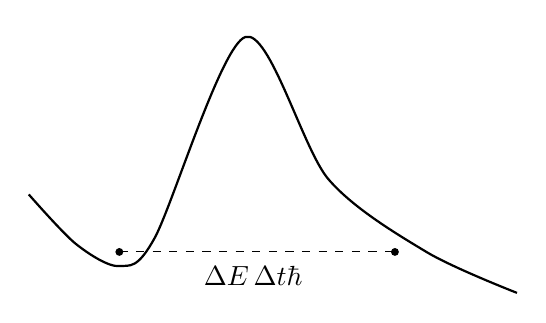
\begin{tikzpicture}[scale=1.0]
\draw[thick] plot[smooth] coordinates {(0.4,1.45) (1.0,0.82) (1.55,0.54) (2.0,0.9) (3.15,3.45) (4.2,1.65) (5.45,0.72) (6.6,0.2)};
\draw[dashed] (1.55,0.72) -- (5.05,0.72);
\fill (1.55,0.72) circle (0.05);
\fill (5.05,0.72) circle (0.05);
\node at (3.25,0.42) {$\Delta E\,\Delta t \lesssim \hbar$};
\end{tikzpicture}
\caption{A schematic redraw of the tunneling analogy: the marked points have the same total energy, while the barrier region represents the classically forbidden intermediate stage.}
\end{figure}

The transfer back to beta decay is immediate. There is simply not enough energy in a neutron to emit a real \(W\) and let it fly off. What can happen is a brief virtual emission. The \(W\) then has to disappear quickly: it may be reabsorbed, or it may turn into lighter final particles such as \(e^-+\bar{\nu}_e\). In the lecture's language, the heavy \(W\) under the propagator is like the particle under the barrier.

Just as important is what \emph{virtual} means. In the lecture's own distinction, real particles are the incoming and outgoing asymptotic states of the process. Virtual particles are the internal lines of the Feynman diagram. They are not directly observed. If one tries to observe them, one must inject enough energy and enough time resolution to change the problem. A probe sharp enough to resolve the short time \(\Delta t\) also carries enough energy to create the corresponding real particle. One no longer has the same process; one has turned the virtual line into a final, real \(W\).

This is why the lecture insists that exact energy conservation is never abandoned. Between the full initial state and the full final state, conservation is exact. The apparent violation belongs only to the intermediate description.

The audience discussion then sharpens one more point. A real \(W\) is not governed by the uncertainty time \(\hbar/\Delta E\) of the virtual process. It has its own short proper lifetime, and if it is produced with large momentum it exhibits ordinary time dilation. Weak lifetimes are long only when the process is forced to proceed through a heavy virtual \(W\) at low energy.

At this stage the lecture also summarizes rate suppression in a useful way. Three ingredients matter:
\begin{itemize}
\item coupling constants,
\item propagators, hence masses and momentum dependence,
\item available energy.
\end{itemize}
In ordinary neutron beta decay, the central suppression is the second of these.

\section{The Missing Third Weak Boson}

Once the discussion of weak rates and virtual exchange has been completed, the lecture briefly returns to the symmetry structure. This is not an afterthought. It is a reminder that the group theory has not yet been fully closed.

If the weak interaction is governed by \(SU(2)\), then the number of weak gauge bosons must match the number of generators. But
\begin{equation}
\dim SU(2)=3.
\end{equation}
So \(W^+\) and \(W^-\) cannot be the whole story. Two charged bosons are not enough. There must be a third weak gauge boson, neutral rather than charged. The lecture does not work it out here; it points forward instead, saying that the missing boson is closely related to the \(Z\), and that the precise relation among \(SU(2)\), \(U(1)\), electric charge, and the neutral weak boson will be taken up next time.

This short return matters because it prevents the opening table picture from hardening too early into a complete theory. The lecture keeps reminding us that the real electroweak structure is a little subtler than the first pass suggests.

\section{Spontaneous Symmetry Breaking}

Only late in the lecture does the subject change, and even then the change is really a bridge to the next lecture. We are not given the Higgs mechanism. We are given the minimal qualitative structure that will later make the Higgs mechanism intelligible.

The first illustration is the dinner-table story. A perfectly symmetric arrangement admits two equally natural choices, left and right. Nothing in the local setup prefers one over the other. But the arrangement is unstable, and once one choice is initiated, the whole system settles that way. The illustration is intentionally informal, but it prepares the right intuition.

Then the lecture gives a more mathematical toy model. Take a lattice of two-state objects; they may be spins, but for the moment they may just as well be classical coins showing heads or tails. Neighboring variables prefer to align, so that
\begin{equation}
E_{\text{parallel}} < E_{\text{anti-parallel}}.
\end{equation}
The lowest-energy configurations are therefore the uniformly aligned ones. But there are two of them:
\begin{equation}
E(\text{all heads}) = E(\text{all tails}).
\end{equation}
So the system has two degenerate ground states.

Now comes the characteristic move. If far away one of the coins is fixed to be heads, that tiny distant asymmetry can select the all-heads ground state. Once that choice has been made, local excitations are measured relative to it. In particular, a tail inserted into a sea of heads costs energy:
\begin{equation}
E(\text{one tail in a sea of heads}) > E(\text{all heads}).
\end{equation}
The microscopic rules were symmetric, but the state that the system chose was not. That is the basic phenomenon of spontaneous symmetry breaking.

\subsection{Question \& Answer}

\paragraph{Question.} How is spontaneous symmetry breaking different from explicit symmetry breaking?

\paragraph{Answer.} In explicit symmetry breaking the local rules are already biased. If a single head simply had lower energy than a single tail, then the symmetry would be broken in the Hamiltonian itself, and there would be only one preferred vacuum. In spontaneous symmetry breaking the local rules remain symmetric, the vacua remain degenerate, and it is the choice of ground state that breaks the symmetry.

The lecture then gives the clean diagnostic. Suppose one insists that very far away on one side the system is heads, and very far away on the other side it is tails. If the breaking is spontaneous, the minimum-energy configuration contains an interface between the two regions. That interface is a domain wall. Domain walls are therefore the qualitative signal of spontaneous, rather than explicit, symmetry breaking.

This is where the lecture stops, and it is wise to let it stop there. The ending is intentionally qualitative. It leaves us with a symmetric local theory, a degenerate family of vacua, an instability that selects one of them, and the preview that the Higgs phenomenon belongs precisely to this class of ideas.

\section{Summary}

The lecture opens by rebuilding the Standard Model from the fermion table outward. \(SU(3)\) acts vertically on color, \(SU(2)\) acts horizontally on weak doublets, and \(U(1)\) acts by phase. The weak interaction is then made concrete through neutron beta decay and through the observation that the same \(W\) structure acts across quark and lepton families when the charge difference is right.

The central question is then posed in the right form: if \(g_w\) is not especially small, why are weak interactions weak? The answer comes from the propagator of a massive exchanged particle. In the lecture's low-energy convention,
\[
\widetilde{\Delta}_W(k)=\frac{1}{k^2+m_W^2},
\]
so at low momentum
\[
\mathcal{A}_{\text{weak}} \sim \frac{g_w^2}{m_W^2},
\qquad
P_{\text{weak}} \sim \frac{g_w^4}{m_W^4}.
\]
That is the spine of the lecture.

After the estimate, the lecture turns interpretive again. A heavy \(W\) can appear only virtually, for a short time, and the tunneling analogy makes that statement intelligible while exact initial-to-final energy conservation remains untouched. Only then does Susskind return briefly to the unfinished electroweak group structure, noticing that \(SU(2)\) should have a third gauge boson. The final turn is qualitative: spontaneous symmetry breaking, degenerate vacua, and domain walls as the signal that the symmetry was broken by the choice of ground state rather than by an explicit local bias. The next lecture will pick up both loose threads: the \(Z\) boson and the Higgs phenomenon.